\documentclass[twocolumn,apj]{openjournal}
\usepackage{amsmath,booktabs}
\usepackage{hyperref}
\hypersetup{colorlinks=true,citecolor=blue,linkcolor=blue,urlcolor=blue,pdfauthor={Kaan Boge}}
\graphicspath{{figures/}}
\renewcommand{\dblfloatpagefraction}{0.65}
\renewcommand{\floatpagefraction}{0.65}
\renewcommand{\dbltopfraction}{0.95}
\renewcommand{\topfraction}{0.95}
\renewcommand{\textfraction}{0.05}
\submitted{}
\makeatletter
\renewcommand{\frontmatter@title@above}{\vspace*{-\headsep}\vspace*{\headheight}\vspace*{0.625in}}
\makeatother
\shorttitle{Cloud survival in supersonic winds}
\shortauthors{Boge}
\begin{document}
\title{Cloud survival in supersonic winds: numerical sensitivity of three-dimensional hydrodynamic calculations}
\author{Kaan Boge}
\affiliation{Independent Researcher}
\begin{abstract}
Cold gas carried through a hot galactic wind can be compressed, accelerated and dispersed, changing the supply and observable distribution of gas around galaxies. Predicting its survival requires understanding how numerical methods represent the interaction between the two phases. We compare three-dimensional cloud-wind calculations using twelve hydrodynamic methods for a reference cloud-to-wind density contrast of 100, with additional grid calculations at contrasts of 10 and 1000. The wind is supersonic, with Mach number 2; the finest initial sampling contains 4,194,304 cells or gas elements, equivalent to about $161^3$. Late-time morphology and dense-gas histories show substantial differences among the recorded configurations. At our finest GIZMO sampling, the meshless finite-mass and finite-volume methods retain 97.6 and 36.7 per cent, respectively, of their initial dense-gas mass after five cloud-crushing times. Their intermediate-temperature gas covers similar projected areas despite this much larger difference in dense mass. The finite-volume mass history also changes non-monotonically with resolution. These results make the treatment of the cloud-wind interface a central target for controlled comparison. Differences in initial particle sampling and wind boundaries must be resolved to connect the numerical spread to reliable predictions of cloud survival.
\end{abstract}
\keywords{hydrodynamics --- instabilities --- methods: numerical --- ISM: clouds --- galaxies: evolution}
\maketitle

\section{Introduction}
Galaxies exchange mass, metals and energy with their surroundings through accretion, outflows and recycling. The circumgalactic medium is a substantial gas reservoir in this cycle, with cool and highly ionized material probed along different sightlines \citep{Tumlinson2017}. Absorption-line measurements in the COS-Halos survey establish the widespread presence of cool, photoionized gas around galaxies and show that its inferred density need not follow a simple two-phase pressure-equilibrium model \citep{Werk2014}. Explaining the persistence and spatial distribution of such material requires understanding how dense gas interacts with hotter surroundings. An isolated cloud in a wind provides a tractable experiment for studying that interaction, although it does not reproduce the full structure of a galactic halo.

Classical shock-cloud calculations linked compression, deformation and disruption to a characteristic cloud-crushing time \citep{Klein1994}. Wind calculations extend this problem to sustained momentum transfer: the cloud must gain speed while shocks and interface disturbances redistribute its mass. Radiative simulations demonstrate that both acceleration and mass loss depend on the wind conditions \citep{Scannapieco2015}, while calculations resolving a broad range of thermal phases show that cloud disruption transfers mass and momentum throughout the resulting multiphase flow \citep{Schneider2017}. These studies motivate following the morphology and velocity of selected gas alongside its remaining dense mass. Here $t_{\rm cc}=\sqrt{\chi}R/v_{\rm w}$, where $R$ is the initial cloud radius, $v_{\rm w}$ is the initial wind speed, and $\chi=\rho_{\rm c,0}/\rho_{\rm w,0}$ is the initial density contrast. Times are expressed in this fixed initial unit.

Cooling can alter the direction of mass exchange between phases. Simulations of fountain clouds show that interaction with cooler, enriched material can promote condensation from a hot corona \citep{Armillotta2016}. In cloud-wind calculations, sufficiently rapid cooling of intermediate-temperature gas can support cold-gas growth and entrainment \citep{GronkeOh2018}; the growth and destruction regimes also depend on the surrounding flow and magnetic fields \citep{Sparre2020}. Thermal conduction supplies another competing process, capable of evaporating cloud gas while compressing some clouds into longer-lived structures \citep{Bruggen2016}. A comparison of hydrodynamic methods must therefore distinguish uncertainty in numerical transport from the effects of these additional physical processes. Our principal sample is non-radiative; the supplementary cooling experiments retain their own resolution and algorithmic qualifications.

Observables place complementary demands on these calculations. Gas mass in a temperature interval does not uniquely determine the area, column density or velocity distribution seen in projection. Conversely, similar projected areas can hide differences in the mass and thermodynamic structure along a sightline. Inferring an ionic absorption signal requires composition, ionization and radiation assumptions in addition to the hydrodynamic fields \citep{Werk2014}. We therefore use column-density morphology and phase-based diagnostics to characterize the simulated gas, without treating a temperature selection as a synthetic ion measurement. The simulations are three-dimensional, allowing disturbances and fragments to evolve in both transverse directions.

The numerical representation of a density interface is a longstanding concern. \citet{Agertz2007} demonstrated substantial differences between grid methods and the standard smoothed-particle hydrodynamics (SPH) formulations in their comparison. Modern algorithms provide several distinct treatments of fluid motion and inter-element transport. Arepo solves finite-volume equations on a moving Voronoi mesh \citep{Springel2010}; GIZMO's meshless finite-mass (MFM) and finite-volume (MFV) methods use a meshless volume partition and Riemann-solver fluxes \citep{Hopkins2015}. MFM and MFV differ in whether mass is exchanged between elements. The presence of moving elements alone does not make these schemes equivalent to one another or to SPH, and their names do not specify a common interface resolution.

\citet{Braspenning2023} compared seven non-radiative hydrodynamic methods using dense-gas mass, intermediate-temperature mass and covering fraction. Their results demonstrate that convergence and agreement depend on the diagnostic, motivating a comparison that goes beyond a single survival curve. We adopt this diagnostic emphasis while reporting the differences between our configurations and theirs explicitly. In particular, the relation between particle construction and spatial sampling must be established before a numerical discrepancy can be interpreted as a disagreement between algorithms.

The present study assembles twelve methods across eleven code implementations, including Arepo, eight grid codes, GIZMO MFM and MFV, and GADGET-4. The reference sample has $\chi=100$ and two common initial samplings; finer sequences extend five methods, and additional grid calculations reach $\chi=10$ and 1000. Its contribution is the joint record of morphology, mass evolution and selected kinematic and thermal diagnostics across this set of configurations. The current boundary and initialization differences limit a solver-only interpretation. The unusual MFV resolution sequence and the changing Arepo endpoint identify concrete targets for controlled follow-up, rather than establishing a uniquely correct method or an exhaustive claim of novelty.

Section~\ref{sec:methods} describes the setup and measurements. Section~\ref{sec:results} presents morphology first, followed by mass evolution and the additional diagnostics. Section~\ref{sec:discussion} examines the MFV and Arepo results in relation to particle spacing, numerical support and transport. The appendices retain numerical validation and the supplementary cooling comparisons, including their unresolved physical and algorithmic limitations.

\section{Methods}\label{sec:methods}
\subsection{Cloud and wind}
We place a spherical cloud in a uniform supersonic wind. The gas has adiabatic index $\gamma=5/3$, and the intended initial cloud and wind are in thermal pressure equilibrium. The reference density contrast is $\chi=100$; the additional grid sequences use $\chi=10$ and 1000. With $r$ measured from the cloud centre, the initial density is
\begin{equation}
\rho(r)=\rho_{\rm w,0}\left[1+\frac{\chi-1}{2}\left(1-\tanh\frac{r-R}{0.1R}\right)\right].
\label{eq:profile}
\end{equation}
The initial velocity is zero within $1.3R$ and equals the wind velocity outside this radius \citep[see also the initial velocity setup in][]{Gronnow2018}. This prescription is used consistently in the primary figures. The wind Mach number is $\mathcal M=v_{\rm w}/c_{\rm s,w}=2$. The simulations evolve to $5t_{\rm cc}$, with scalar histories normally sampled every $0.05t_{\rm cc}$.

The domain extends from $-3R$ to $17R$ along the wind and from $-5R$ to $5R$ in both transverse directions. Grid wind-tunnel configurations impose upstream inflow and downstream outflow. The archived Arepo setup is periodic along the wind, and the GIZMO and GADGET-4 setups are fully periodic. These boundary choices determine how gas and disturbances can leave or re-enter the domain and are retained when interpreting the results. Pressure reconstruction is a further distinction: GADGET-4's initial peak pressure exceeds the intended value by factors of about 3.90 and 2.10 at the two common samplings. Its curves are included as a diagnostic case, with this departure identified in the figure caption.

\subsection{Spatial resolution and particle construction}
We denote initial sampling by $n$, the number of intervals across a transverse side of length $10R$. The corresponding uniform grid has $2n\times n\times n$ cells, and its spacing is $\Delta x=10R/n$. Table~\ref{tab:resolution} gives both the spacing and the equivalent cubic count, $N^{1/3}$, where $N=2n^3$. The full twelve-method comparison uses $n=32$ and 64; the available finer sequences use $n=128$.
\begin{table}[tb]
\centering
\caption{Initial sampling in the $20R\times10R\times10R$ domain. $N^{1/3}$ is the side count of a cube containing the same number of cells or initial lattice points.}
\label{tab:resolution}
\begin{tabular}{rrrr}
\toprule
$n$ & Domain sampling & $\Delta x/R$ & $N^{1/3}$\\
\midrule
32 & $64\times32\times32$ & 0.3125 & 40.3\\
64 & $128\times64\times64$ & 0.15625 & 80.6\\
128 & $256\times128\times128$ & 0.078125 & 161.3\\
\bottomrule
\end{tabular}
\end{table}

The finest GIZMO calculations contain 4,194,304 gas elements. Their initializer uses a uniform lattice with variable particle masses $m_i=\rho(r_i)\Delta x^3$. Thus the density contrast is represented by a mass contrast at common initial spacing. The saved preparation record confirms a cloud-to-wind particle-mass ratio approaching 100 and 8,808 particle centres inside $r\leq R$ for the reference case. The input internal energy is assigned from the intended uniform pressure. The solver subsequently reconstructs density from its own volume or kernel estimate, making the reconstructed initial pressure an important diagnostic.

The meshless spatial distribution evolves with the flow. Consequently, the initial spacing specifies the starting sample, whereas the later effective resolution also depends on the local element distribution and reconstruction. The initial density transition has width $0.1R$, corresponding to 1.28 uniform-grid spacings at $n=128$. This narrow interface remains a demanding part of the resolution study.

\subsection{Hydrodynamic methods and comparison groups}
The grid-based sample comprises Athena++ \citep{Stone2020}, AthenaPK on the Parthenon framework \citep{Grete2022}, Athena 4.2 \citep{Stone2008}, Enzo \citep{Bryan2014}, Enzo-E/Cello \citep{Bordner2018}, RAMSES \citep{Teyssier2002}, FLASH 4.8 \citep{Fryxell2000} and Flash-X \citep{Dubey2022}. The remaining methods are the moving-mesh code Arepo \citep{Springel2010}, GIZMO MFM and MFV \citep{Hopkins2015}, and the SPH implementation in GADGET-4 \citep{Springel2021}. MFM and MFV are two methods in one code, giving twelve methods across eleven code implementations.

The reference mass comparison uses $\chi=100$ at $n=32$ and 64 for all twelve methods. Athena++, Enzo, Enzo-E and both GIZMO methods also have $n=128$ histories in this comparison. The contrast extension contains $n=128$ results for Enzo and Enzo-E at $\chi=10$ and 1000, Athena++ at $\chi=10$ and 1000, and AthenaPK at $\chi=10$. Each curve is associated with its actual numerical configuration. The common analytic profile and nominal sampling provide a starting point for comparison; matching the wind boundaries and reconstructed initial pressure is required for a solver-only interpretation.

We use the published method papers to identify the algorithms, while the saved inputs define the particular calculations. A code name alone does not specify its Riemann solver, reconstruction or diffusion options. Changes to those options require a new calculation. The earlier supplementary AthenaPK pair uses HLLE fluxes, piecewise-linear reconstruction (PLM) and van Leer integration. Its non-radiative $\chi=10$ extension uses the same modified flux correction, with four final fallback activations. Additional completed AthenaPK calculations use HLLC fluxes and piecewise-parabolic reconstruction (PPM): non-radiative $\chi=10$ and 100, and radiative $\chi=100$. The correction source and fallback history distinguish these configurations, as detailed in Appendix~\ref{app:hllc}.

\subsection{Measurements}\label{sec:measurements}
Dense gas is selected by $\rho>\rho_{\rm c,0}/3$. We sum its mass and normalize by the measured initial dense mass of the same calculation, giving $f_{\rm d}(t)=M_{\rm d}(t)/M_{\rm d}(0)$. This measures the mass satisfying a density criterion at each time. Compression and thermal evolution can change membership of that selection, so an increase in $f_{\rm d}$ can occur during compression.

Morphology panels show total-gas column density integrated along the line of sight, normalized by $\rho_{\rm c,0}R$. Edge-on and face-on views use the same domain and explicitly stated colour scale. Grid columns are computed by summing cell contributions. GIZMO images deposit particle masses at their centres on a common image grid. The visualization conserves the deposited mass; its pixel-scale appearance also reflects the chosen deposition scheme. Appendix~\ref{app:validation} describes checks on these reductions.

For the finest MFM and MFV calculations, 11 states separated by $0.5t_{\rm cc}$ provide additional diagnostics. We measure the mass-weighted streamwise velocity of the dense selection. Intermediate-temperature gas is selected using $\chi^{-3/4}<T/T_{\rm w,0}<\chi^{-1/4}$, following the temperature-band diagnostic of \citet{Braspenning2023}. Its mass is normalized by $M_{\rm d}(0)$. For fixed composition, temperature is proportional to specific internal energy; the corresponding grid expression uses $P/\rho$.

The intermediate-temperature covering fraction is the fraction of the full transverse domain above column threshold $0.01(2\rho_{\rm c,0}R)$. We use a $128^2$ image grid. Applying the same column threshold to dense gas gives an area $A_{\rm d}$ and a projected effective radius $R_{\rm eff}=\sqrt{A_{\rm d}/\pi}$. The mean dense-gas contrast is $\chi_{\rm eff}=M_{\rm d}/(\rho_{\rm w,0}V_{\rm d})$, with $V_{\rm d}=\sum_{\rm dense}m_i/\rho_i$. Together with the measured velocity, these give
\begin{equation}
t_{\rm cc,eff}(t)=\frac{\sqrt{\chi_{\rm eff}(t)}R_{\rm eff}(t)}{|v_{\rm w}-\langle v_\parallel\rangle_{\rm d}(t)|}.
\label{eq:effective}
\end{equation}
This diagnostic combines the evolving size, density and relative speed using the imposed initial wind as reference. It characterizes the selected gas at each time; determining a disruption time requires following its subsequent evolution. Initial projection and selection effects can make $R_{\rm eff}(0)$ differ from $R$. GIZMO velocities retain their native time staggering.

\section{Results}\label{sec:results}
\subsection{Late-time morphology}
Figure~\ref{fig:morph} shows the grid overview at $n=64$, and Figure~\ref{fig:morphnew} presents the finer GIZMO states alongside the available Enzo contrast endpoints. The maps reveal differences in the concentration of the cloud, the extent of its wake and the structure transverse to the wind. Several grid calculations retain a bright leading concentration with a fainter wake. Their face-on views display different rings and angular features. Morphology therefore adds information beyond the amount of gas above a density threshold.

The $\chi=10$ Enzo cloud remains comparatively coherent at the final time, while the $\chi=1000$ map has a more irregular and extended distribution. The ambient column contributes more strongly to the normalized low-contrast image because $\rho_{\rm w,0}/\rho_{\rm c,0}$ is larger. The same colour normalization can consequently display different background brightness even when the wind density convention is unchanged.

The MFM and MFV maps both show asymmetric structure at $n=128$. Their projected appearance accompanies a much larger difference in dense mass, quantified below. Fine granularity in the meshless images depends on particle-centre deposition, whereas the larger features reflect the mass distribution across many pixels. A comparison of slices and kernel-smoothed projections would help separate the influence of visualization from the underlying structure.
\begin{figure*}[tp]
\centering
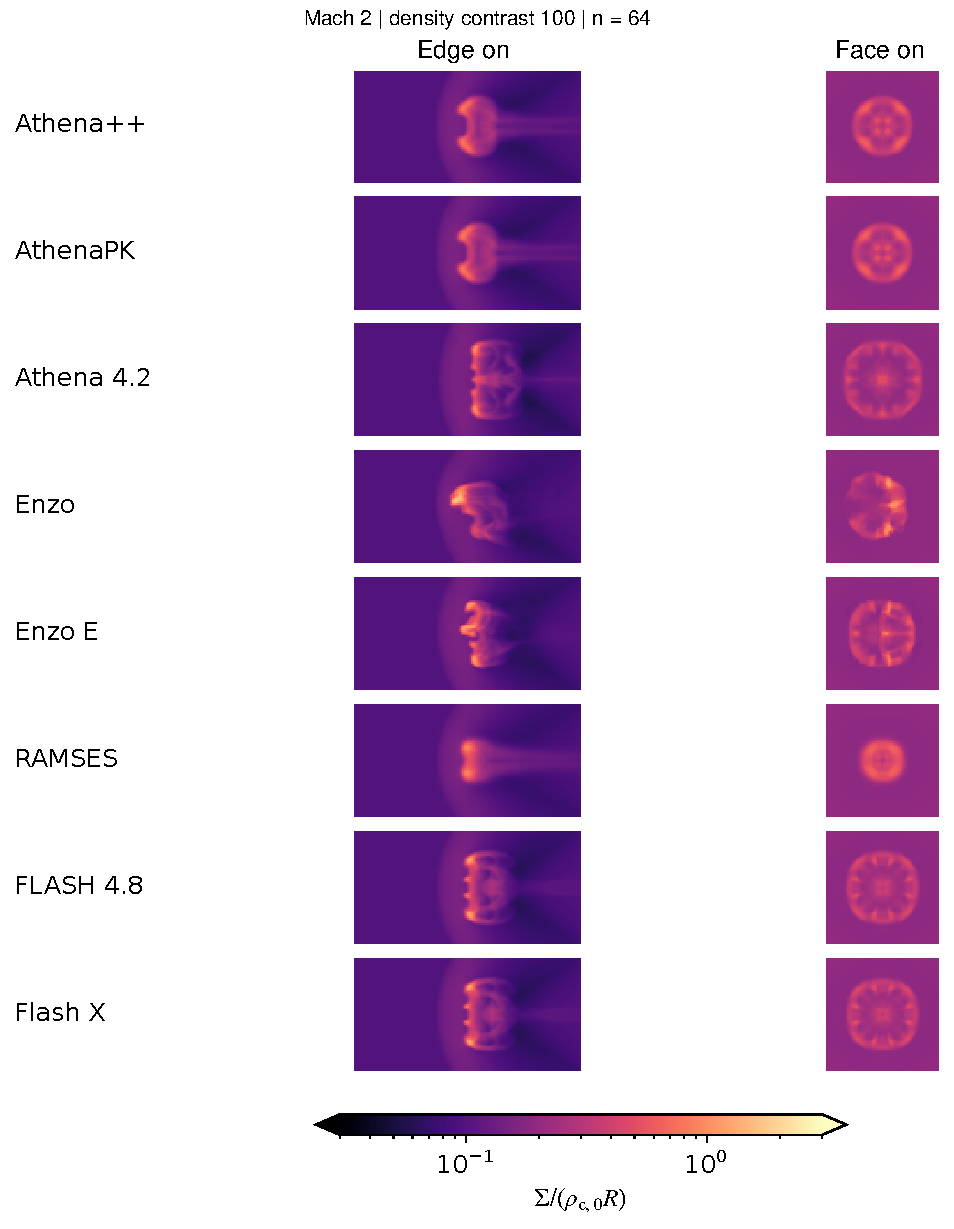
\includegraphics[width=.82\textwidth,height=.69\textheight,keepaspectratio]{morphology.pdf}
\caption{Total-gas column density at $t\simeq5t_{\rm cc}$ for the grid reference sample, with $\chi=100$, $\mathcal M=2$ and initial sampling $128\times64\times64$ ($n=64$). Rows identify the methods; columns give edge-on and face-on views. All panels use the same logarithmic scale and full domain.}
\label{fig:morph}
\end{figure*}
\begin{figure*}[tp]
\centering
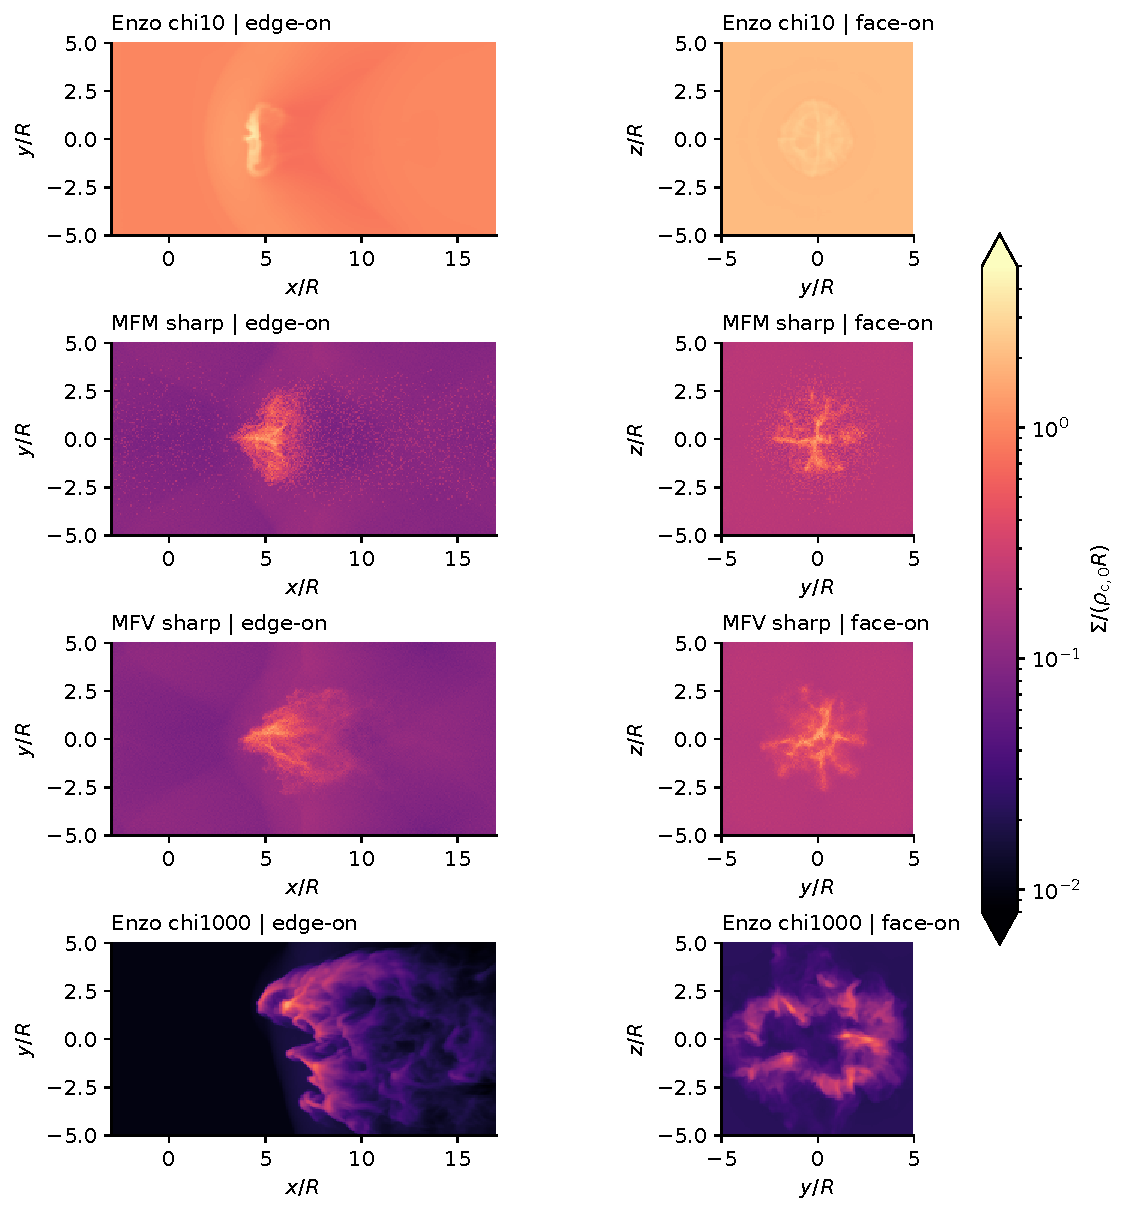
\includegraphics[width=.94\textwidth,height=.68\textheight,keepaspectratio]{late_morphology_new.pdf}
\caption{Finer morphology at $5t_{\rm cc}$ and initial sampling $256\times128\times128$ ($n=128$). Enzo illustrates contrasts of 10 and 1000; GIZMO MFM and MFV illustrate contrast 100. The colour scale is $0.008\leq\Sigma/(\rho_{\rm c,0}R)\leq5$, with end triangles indicating saturation. GIZMO uses particle-centre deposition and periodic boundaries; Enzo uses cell sums and an open wind setup.}
\label{fig:morphnew}
\end{figure*}

\subsection{Dense-gas survival and resolution}
Figure~\ref{fig:mass} compares the reference histories at their available resolutions. At $n=128$, MFM retains 97.6 per cent of its initial dense mass at $5t_{\rm cc}$, while MFV retains 36.7 per cent. Refinement from $n=64$ changes their final fractions from 0.965 to 0.976 and from 0.409 to 0.367, respectively. The two methods thus remain well separated after this refinement step.

Across the three initial samplings, the MFM endpoints are approximately 0.971, 0.965 and 0.976. MFV gives 0.253, 0.409 and 0.367. The MFV sequence is non-monotonic: the increase between the two coarser calculations reverses at the next resolution. A trend inferred only from the first pair would miss this change. MFM's dense fraction is more stable over the tested range, while convergence of other quantities must be assessed separately.

Over the full histories, the maximum $n=64$ to 128 difference is 1.96 percentage points for MFM and 11.25 points for MFV. The corresponding differences for Athena++, Enzo and Enzo-E are 22.05, 5.93 and 10.80 points. These numbers describe deterministic differences between resolutions. Their scale and the narrow initial interface motivate further refinement and controlled initialization tests.
\begin{figure*}[tp]
\centering
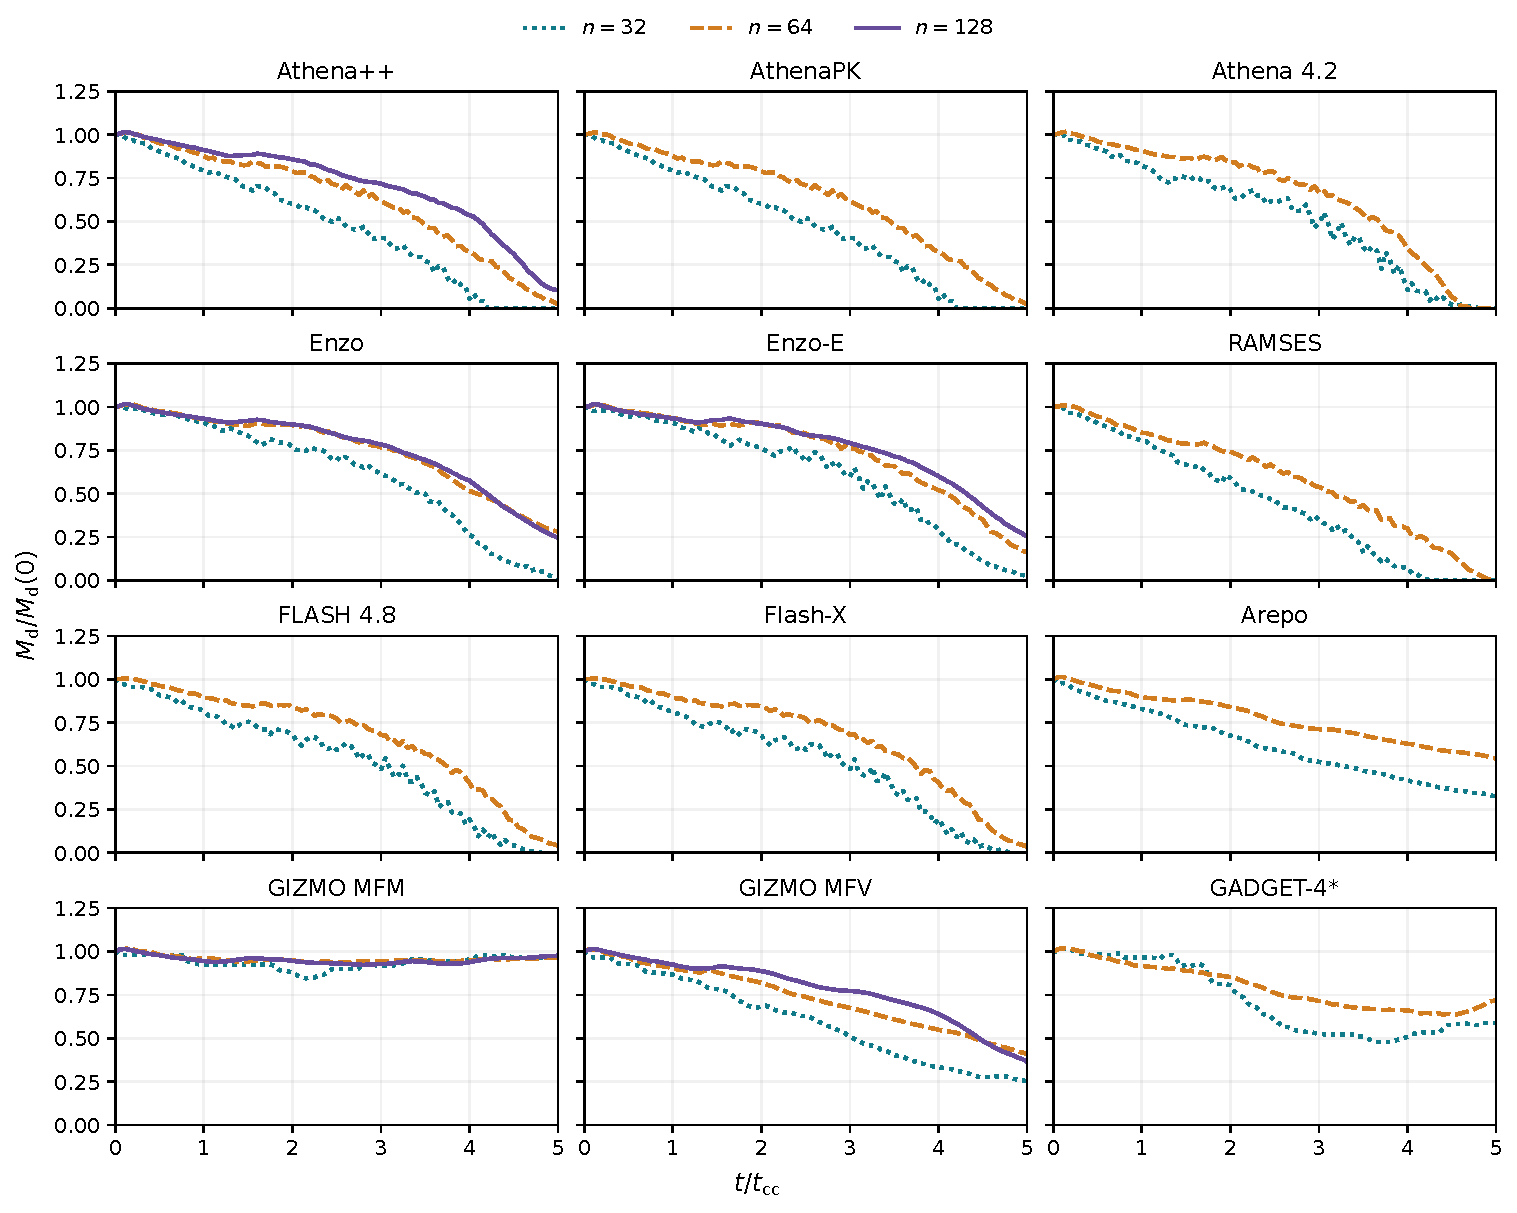
\includegraphics[width=\textwidth,height=.68\textheight,keepaspectratio]{mass_histories.pdf}
\caption{Dense-gas histories at $\chi=100$ and $\mathcal M=2$. Line styles identify the initial transverse sampling $n=32$, 64 and 128; domain dimensions are $2n\times n\times n$. MFM and MFV are placed together for comparison. All twelve methods have the two coarser histories; five have the finer extension. GADGET-4 is marked with an asterisk because its initial reconstructed peak pressure differs from the intended equilibrium. The wind-boundary differences are specified in Section~\ref{sec:methods}.}
\label{fig:mass}
\end{figure*}

The moving-mesh Arepo histories also change substantially with refinement. Their final dense fractions increase from 0.325 at $n=32$ to 0.543 at $n=64$, a difference of 21.8 percentage points. At the common $n=64$ sampling, the Arepo endpoint lies between those of MFV (0.409) and MFM (0.965). This ordering is a measurement of the saved configurations, which have different boundary choices. There is no accepted $n=128$ Arepo history in this comparison, so its coarse-to-fine increase does not establish a converged trend.

The supplementary initial-velocity controls give final dense fractions of 0.978 for MFM and 0.334 for MFV at $n=128$. The method-to-method separation remains large in those controls. They are retained as supporting measurements in Appendix~\ref{app:validation}, while the main figures use a single velocity prescription. 

\subsection{Density contrast}
The grid contrast histories are shown in Figure~\ref{fig:contrast}. At $\chi=10$, the final dense fractions are 0.722 for Enzo, 0.734 for Enzo-E, 0.621 for Athena++. AthenaPK gives 0.565 with the earlier HLLE/PLM configuration and 0.463 with the HLLC/PPM configuration. Both retain their initial tagged-material integral at the endpoint. Their modified corrections triggered four and 130 global first-order fallback stages, respectively. This numerical-configuration sensitivity accompanies changes in reconstruction, fluxes and correction source, whose individual effects require separate controls. At $\chi=1000$, Enzo and Enzo-E give 0.169 and 0.171, whereas the additional Athena++ calculation gives 0.0721. The latter uses $n=128$ with 16 mesh blocks and retains 86.2 per cent of its initial tagged-material integral and 92.5 per cent of its initial total domain mass at $5t_{\rm cc}$. Dense-gas membership therefore changes much more than the tagged-material integral in this calculation. These three measures are distinct: a dense-mass decrease alone does not separate mixing, dilution and transport through the boundaries. The larger spread in the high-contrast dense fractions motivates matched transport and boundary controls; it does not identify one method as physically correct.

The normalization by $t_{\rm cc}$ accounts for the initial contrast in the shock-crossing scale. For fixed radius and wind speed, the high-contrast calculation reaches a given $t/t_{\rm cc}$ after a longer absolute time. At $5t_{\rm cc}$, the $\chi=1000$ evolution has lasted ten times as long as the $\chi=10$ evolution. This distinction matters for the time available for transport through a finite domain.

Retained cloud-tag integrals, where available, provide a separate measure of material remaining in the domain. In the high-contrast Enzo calculation, 81.4 per cent of the initial tracer integral remains at the endpoint while only 16.9 per cent of the initial dense mass remains. Much of the tagged material can therefore occupy gas below the density threshold. A complete boundary flux budget would quantify the contribution of material leaving the domain.
\begin{figure*}[tp]
\centering
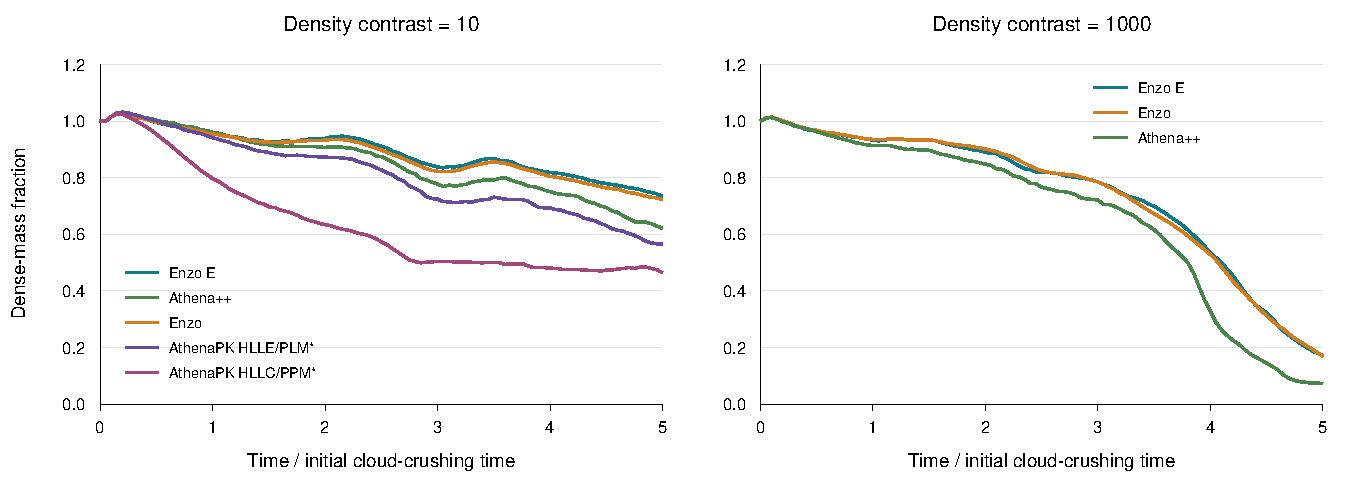
\includegraphics[width=.94\textwidth]{contrast_histories_updated.pdf}
\caption{Available $n=128$ grid histories at contrasts of 10 and 1000, all with a Mach 2 wind. The denominator is each calculation's measured initial dense mass. The AthenaPK curves, marked with asterisks, use the modified corrections discussed in Appendix~\ref{app:cooling} and represent separate numerical configurations. These panels extend the contrast range of the reference comparison.}
\label{fig:contrast}
\end{figure*}

\subsection{Velocity, thermal phases and projected structure}
Figure~\ref{fig:diagnostics} compares the finer MFM and MFV runs using the same density and temperature selections. At $5t_{\rm cc}$, the mass-weighted dense-gas velocities are $0.328v_{\rm w}$ and $0.208v_{\rm w}$, respectively. The velocity describes the selected gas at each time; its evolution includes changes in membership as material crosses the density threshold.

The intermediate-temperature masses are 0.444 and 0.501 times the initial dense mass for MFM and MFV. The projected covering fractions are 0.201 and 0.184. Thus a large difference in dense mass accompanies relatively similar intermediate-temperature projected areas. Mass and covering fraction respond differently to how gas is distributed in temperature, density and space, making both useful for connecting the calculation to observable columns.

The dense-gas projected radii reach $2.62R$ and $1.57R$, and the mean selected contrasts are 74.6 and 63.9. Combined with the relative wind speed, these yield $t_{\rm cc,eff}=3.37t_{\rm cc}$ and $1.59t_{\rm cc}$ for MFM and MFV. The component panels show how the larger MFM projected area and its smaller relative wind speed contribute to that difference. Fragmentation and overlap along a viewing direction also affect the inferred area. The timescale is consequently interpreted together with its density, size and velocity factors.
\begin{figure*}[tp]
\centering
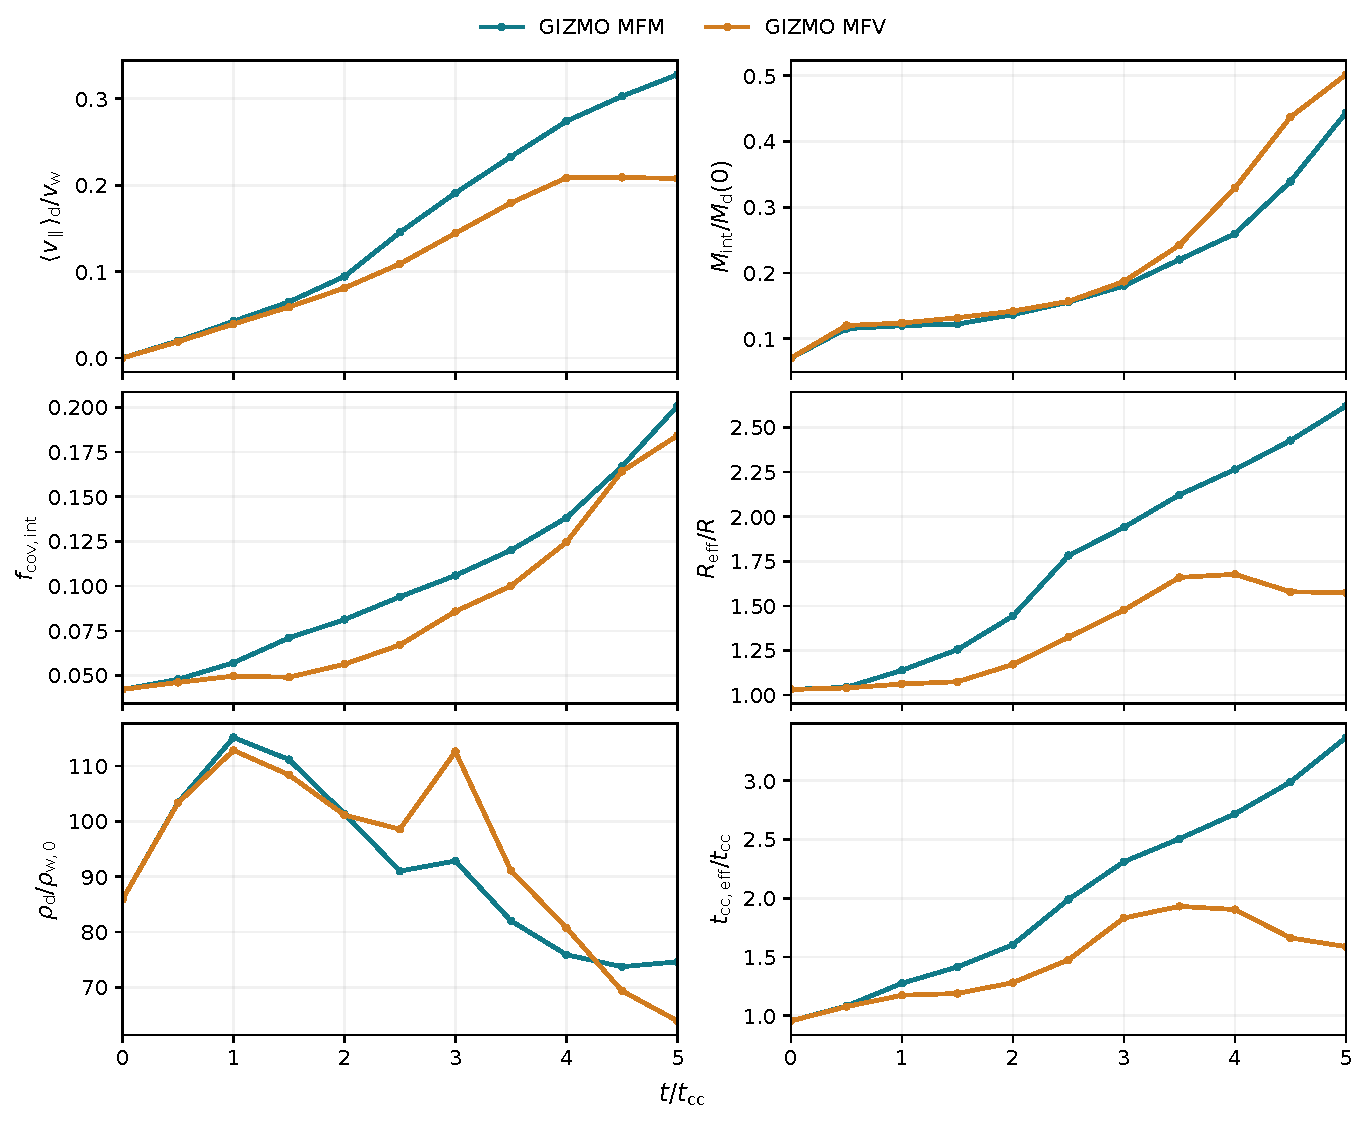
\includegraphics[width=.95\textwidth,height=.68\textheight,keepaspectratio]{gizmo_diagnostics.pdf}
\caption{Kinematic, thermal and geometric diagnostics of the non-radiative GIZMO calculations at $n=128$ and $\chi=100$. Points represent 11 saved states separated by $0.5t_{\rm cc}$. The intermediate-temperature mass and covering fraction use the same definitions for both methods. The lower panels give the quantities entering Equation~\ref{eq:effective}.}
\label{fig:diagnostics}
\end{figure*}

\section{Discussion}\label{sec:discussion}
\subsection{MFV evolution in relation to previous comparisons}
The GIZMO comparison shows a large separation at the finest sampling: MFM retains 0.976 of its initial dense mass at $5t_{\rm cc}$, whereas MFV retains 0.367. The MFV endpoints, 0.253, 0.409 and 0.367 as $n$ increases, also rule out a simple monotonic extrapolation from the two coarser calculations. These are descriptive results of the recorded configurations. Neither persistence of dense gas nor a small change in one endpoint alone demonstrates an accurate solution of the cloud-wind problem.

Resolution-sensitive MFV evolution is not absent from the literature. \citet{Braspenning2023} found a slower late-time MFV decline at higher resolution for $\chi=10$; at $\chi=100$, their MFM cloud dispersed faster than their MFV cloud, and MFV closely followed Arepo. Our persistent MFM component has the opposite method ordering. Their meshless schemes were independent SWIFT implementations, with Mach 1.5 winds and a $40R\times10R\times10R$ periodic domain, whereas we use GIZMO, Mach 2 and a $20R\times10R\times10R$ domain. This comparison identifies a discrepancy to explain, without attributing it to one method's correctness.

\subsection{Particle spacing and numerical support}
The initialization records identify a specific difference in spatial sampling. Our GIZMO cloud occupies a uniform lattice with variable masses, $m_i=\rho(r_i)\Delta x^3$. The cloud-to-wind mass ratio approaches 100 at the reference contrast. In the equal-mass construction of \citet{Braspenning2023}, the cloud has a greater element number density. At fixed wind spacing, equal-mass sampling at $\chi=100$ gives an idealized cloud spacing smaller by $\chi^{1/3}\simeq4.64$. The same nominal wind resolution therefore need not give comparable resolution of the cloud interior or its interface. This geometric difference is established; its contribution to the measured mass histories remains untested.

Particle spacing must also be distinguished from the numerical support used to reconstruct the fluid. In MFM and MFV the kernel defines a volume partition and a neighbourhood for reconstruction; it does not have the same role as the smoothing kernel in a conventional SPH density estimate \citep{Hopkins2015}. The relevant comparison should record the support-radius distribution, neighbour counts, particle masses and reconstructed density and pressure across the initial interface. Increasing the number of neighbours is not equivalent to increasing spatial resolution, and a smoother rendered image supplies no evidence that the hydrodynamic interface is better resolved.

At $n=128$, the adopted $0.1R$ transition spans only 1.28 initial lattice spacings. A pressure profile assigned from the analytic density can consequently differ from the pressure reconstructed by a particular solver. The GADGET-4 pressure departures demonstrate that this distinction matters in the archive, but do not establish the same error in GIZMO. A controlled MFM--MFV test should compare equal-mass and variable-mass realizations, first matching the wind spacing and then matching the measured interface support. Pressure balance and the first update should be measured in each realization before varying the support prescription. Particle spacing and neighbour support are thus testable explanations for the present discrepancy, not inferred causes.

\subsection{What the Arepo comparison adds}
Arepo supplies a useful comparison because it exchanges mass across explicit moving cell faces \citep{Springel2010}, while MFV uses effective faces defined by its meshless partition \citep{Hopkins2015}. Both can follow the bulk flow while permitting inter-element mass transport. This common feature motivates comparing their phase and mass evolution, but does not require agreement at finite resolution: the volume partition, gradients, motion and regularity of the elements can differ.

The measured Arepo endpoint changes from 0.325 to 0.543 between $n=32$ and 64. At $n=64$ it exceeds the MFV endpoint by 13.3 percentage points, while remaining well below MFM. At this sampling, the methods therefore span more than a simple division between fixed-mass and mass-exchanging schemes. Arepo has only two resolutions in the present sample, and its archived wind-periodic setup differs from the fully periodic GIZMO setup and open grid wind tunnels. The current comparison cannot isolate the moving mesh as the cause of the separation or determine whether refinement would move Arepo toward the finest MFV result.

A matched Arepo extension should measure initial cell-volume and mass distributions, reconstructed pressure, and the resolution of the cloud boundary before following the same dense and intermediate-temperature selections. Matching the domain, boundaries and analytic profile would then make it possible to compare how the different volume partitions transport gas through the interface. Density and temperature structure, covering fraction and mass exchange should be assessed together; matching a final dense fraction could otherwise conceal different phase distributions.

\subsection{Boundary, transport and physical interpretation}
Periodic boundaries can retain material and recirculate disturbances, whereas an open wind tunnel supplies upstream gas and permits downstream loss. The size of the effect depends on the flow, domain and elapsed time; periodicity alone does not explain the present ordering. Boundary mass and energy fluxes, measured alongside the dense component's motion, are needed to separate in-domain dispersal from material leaving the calculation. Matched open and periodic controls would establish the dynamical contribution of these choices.

The completed AthenaPK HLLC/PPM series extends the comparison with the earlier HLLE/PLM calculations. Because reconstruction, Riemann solver and correction source are not all held fixed across those groups, their differences cannot be assigned to a single transport choice. Athena's exact H-correction setting also remains to be verified before identifying the regular structures in Figure~\ref{fig:morph} with a shock instability. A visual resemblance is insufficient to establish that diagnosis.

The MFM--MFV diagnostics illustrate why several measurements are necessary: intermediate-temperature covering fractions remain similar despite a large dense-mass difference. Shocks, adiabatic evolution and numerical mixing can all move non-radiative gas through a temperature selection. Material tags combined with density and temperature would distinguish original cloud gas from ambient material that becomes dense. A measured local ambient velocity would also improve the shear estimate in the evolving cloud-crushing diagnostic. These additions would connect the recorded phase distributions more directly to entrainment and exchange.

For the radiative sample, resolving the cooling layer and distinguishing radiated energy, temperature-floor input and boundary transport remain necessary. The larger dense fractions with cooling are measured outcomes of the stated modified algorithms; a universal cooling-induced survival enhancement cannot be inferred from them. Matched controls and additional methods are needed before extending that interpretation. The highest-priority missing experiments are therefore the particle-construction and support tests, a finer matched Arepo sequence, boundary controls, and separate transport and cooling-resolution tests. They remain future work rather than results of the present comparison.

\section{Conclusions}
Three-dimensional morphology, dense-gas histories and thermal diagnostics reveal a broad spread in the outcomes of the recorded cloud-wind calculations. At $\chi=100$ and the finest GIZMO sampling, MFM retains 97.6 per cent of its initial dense-gas mass after five cloud-crushing times, compared with 36.7 per cent for MFV. The MFV dense-mass sequence is non-monotonic with increasing resolution. Arepo is also resolution sensitive: its final dense fraction rises from 0.325 to 0.543 over the two available samplings, with a finer matched comparison still required. The corresponding intermediate-temperature covering fractions, 0.201 and 0.184, are much closer than the dense-mass fractions.

The additional grid histories extend the comparison to contrasts of 10 and 1000. Enzo and Enzo-E retain approximately 17 per cent of their initial dense mass at the high-contrast endpoint, compared with 7.2 per cent in Athena++. The time histories and available morphology panels provide complementary measures of the evolution; explaining the spread requires the matched controls described above.

Explaining the spread requires a controlled comparison of reconstructed pressure, particle sampling, wind boundaries and numerical transport. The confirmed variable-mass initialization, unresolved interface support and the GADGET-4 pressure departures identify concrete tests. The different MFM--MFV ordering relative to earlier work makes these controls particularly important; no single mechanism has yet been isolated. Establishing the effects of these choices is the next step toward using cloud-wind calculations to infer the survival and observable distribution of cold gas in galactic flows.

\section*{Data and code availability}
The custom source and portable scalar plotting package are available at \url{https://github.com/KaanBoge/cloud-studio/tree/main/code/paper_20261026}. The accompanying source bundle includes the LaTeX manuscript, bibliography, figures, saved scalar and diagnostic series, and figure-generation code. The complete numerical outputs and original configurations are preserved in the research archive. The supplementary documentation records source identifiers and the scope of each comparison. Custom initialization and analysis code, together with documented solver changes, are supplied for reproducibility.

\section*{Acknowledgments}
Generative-AI assistance was used in code development, analysis scripting and manuscript preparation. Checks on the numerical outputs and diagnostic reductions are described in Appendix~\ref{app:validation}. The scientific interpretation and manuscript remain subject to author review.

\bibliographystyle{apsrev4-1}
\bibliography{references}

\appendix
\section{Validation and supporting measurements}\label{app:validation}
Saved results underwent checks of output coverage, cadence, required fields, finite values, density and pressure positivity, and selected mass and scalar integrals. The GIZMO extensions each contain 101 saved states through $5t_{\rm cc}$. The Enzo high-contrast field series was inspected separately after the original controller reported a failure; the saved-data result and the controller outcome remain distinct in the provenance records.

The additional diagnostics reuse 11 saved states per selected calculation. Their dense-mass reductions agree with the previously accepted scalar values, with a maximum recorded relative difference of $2.2\times10^{-16}$. Projected mass sums were checked against the corresponding selected masses. These comparisons test the reductions and data handling. Physical convergence additionally requires a controlled resolution sequence and sensitivity tests of the selection and projection.

The main figures use a single velocity prescription. At $n=128$, the supplementary GIZMO velocity controls have dense fractions of 0.9784 for MFM and 0.3341 for MFV, compared with 0.9760 and 0.3665 in the primary calculations. All four histories are retained in the source bundle. The primary grid and meshless figures, the contrast extension, and the separate cooling pair account for the newly completed results while keeping their comparison groups distinct.

The new non-radiative AthenaPK $\chi=10$ case contains 101 outputs through $5t_{\rm cc}$ and passed the reviewed automatic field and cadence checker. The controller and its output streams closed successfully before integration. Its result is retained with the modified-algorithm limitations above. This adds one completed evolution to the earlier 65-record inventory.

The additional non-radiative Athena++ $\chi=1000$ calculation contains 101 distinct saved states, separated by $0.05t_{\rm cc}$ through $5t_{\rm cc}$. The completion screen covers all 4,194,304 cells, six double-precision fields, the bound initial conditions, finite field values and the saved mass reductions. The original native process exited successfully and its output streams and owned processes were settled before acceptance. This establishes numerical coverage, not physical convergence; restart recovery and new morphology or thermal reductions have not been tested for this series.

Three further HLLC/PPM evolutions each contain 101 accepted saved states through $5t_{\rm cc}$. Their endpoint integrals and scalar histories appear in Appendix~\ref{app:hllc}. The acceptance checks establish numerical coverage and bounded fields; the configuration differences and physical-resolution qualifications remain part of their interpretation.

The original inventory contains 65 completed evolution records across primary calculations and supporting controls. The source bundle retains that inventory as provenance rather than using its count as a measure of parameter coverage. Restart segments, readiness tests and failed attempts are tracked separately. Any newly launched case enters the figures after its numerical validation and analysis have completed.

\section{Supplementary radiative experiment}\label{app:cooling}
\subsection{Physical setup and cooling time}
A separate AthenaPK pair explores radiative cooling at $\chi=100$, $\mathcal M=2$, $R=100$ pc and $n=128$. The wind density and temperature are $10^{-27}$ g cm$^{-3}$ and $10^6$ K; the cloud values are $10^{-25}$ g cm$^{-3}$ and $10^4$ K. The wind speed is 305.76 km s$^{-1}$ and $t_{\rm cc}=3.20$ Myr. The mesh contains 128 blocks of $32^3$ cells. Both runs use open wind boundaries, HLLE fluxes, piecewise-linear reconstruction, van Leer integration and a $10^4$ K temperature floor.

The cooling table uses the solar-abundance equilibrium rates of \citet{Sutherland1993} in the implementation's $n_{\rm H}^2\Lambda(T)$ convention, integrated with the method of \citet{Townsend2009}. The equation of state assumes fully ionized H/He with helium mass fraction $Y=0.24$ and hydrogen fraction $X=0.76$. The mean molecular weight is therefore $\mu=(2X+3Y/4)^{-1}=0.588$. The fixed-composition equation of state and equilibrium cooling table are the adopted approximations.

An isobaric mixed-phase estimate gives $T_{\rm mix}=10^5$ K and $\rho_{\rm mix}=10^{-26}$ g cm$^{-3}$. Using the actual table value $\Lambda(10^5\,{\rm K})=10^{-20.87}$ erg cm$^3$ s$^{-1}$, the thermal-energy cooling time is
\begin{equation}
t_{\rm cool,mix}=\frac{(3/2)n_{\rm tot}k_{\rm B}T_{\rm mix}}{n_{\rm H}^2\Lambda(T_{\rm mix})},
\label{eq:tcool}
\end{equation}
where $n_{\rm tot}=\rho/(\mu m_{\rm p})$ and $n_{\rm H}=X\rho/m_{\rm p}$. This gives approximately 0.24 Myr, or $0.075t_{\rm cc}$. The corresponding sound-crossing cooling length is about 12 pc, compared with a cell size of 7.81 pc. The cooling layer is thus sampled by only about 1.5 cells. This estimate characterizes the chosen mixed-phase state; the evolving flow contains a distribution of cooling times.

\subsection{Material tracer and flux correction}
The additional scalar is an advected cloud-material tag: its mass fraction distinguishes initially cloud-associated gas from ambient wind gas. It is transported with the fluid and measures material origin. The calculations remain in the imposed wind frame. Dense mass and tracer mass answer different questions because the former uses an evolving density threshold and the latter tracks the advected tag.

The custom correction acts on the numerical update when a candidate state violates density, pressure or tracer bounds. Shared interface fluxes are corrected consistently between neighbouring cells. In the last of four correction sweeps, persistent invalid cells trigger a whole-domain update using first-order local Lax--Friedrichs fluxes evaluated from the original stage state. The correction changes the hydrodynamic update during evolution. Both pair members use the same modified algorithm. The final fallback activated 23 times with cooling and 55 times without cooling, and can introduce additional numerical diffusion. The retained source change and activation counts are included in the supplementary code documentation.

\subsection{Pair results}
At $5t_{\rm cc}$, the cooling-on and cooling-off runs retain dense fractions of 0.882 and 0.105. The corresponding tracer fractions are 0.985 and 0.964. Figure~\ref{fig:cooling} shows their morphology and mass histories separately from the cross-code comparison. Figure~\ref{fig:cooldiag} gives the accompanying thermal and kinematic diagnostics.

The intermediate-temperature masses are 0.108 and 0.858 initial dense masses, while the covering fractions are 0.062 and 0.239. The selected dense-gas velocities are $0.278v_{\rm w}$ and $0.351v_{\rm w}$. Cooling changes the distribution among thermal phases substantially in this pair. Interpreting the magnitude requires resolving the cooling layer and measuring the energy supplied by the temperature floor, radiated away and transported through the boundaries. The two fallback activation histories also warrant comparison at higher resolution. The pair is retained as a supplementary pilot with these qualifications.
\begin{figure*}[tp]
\centering
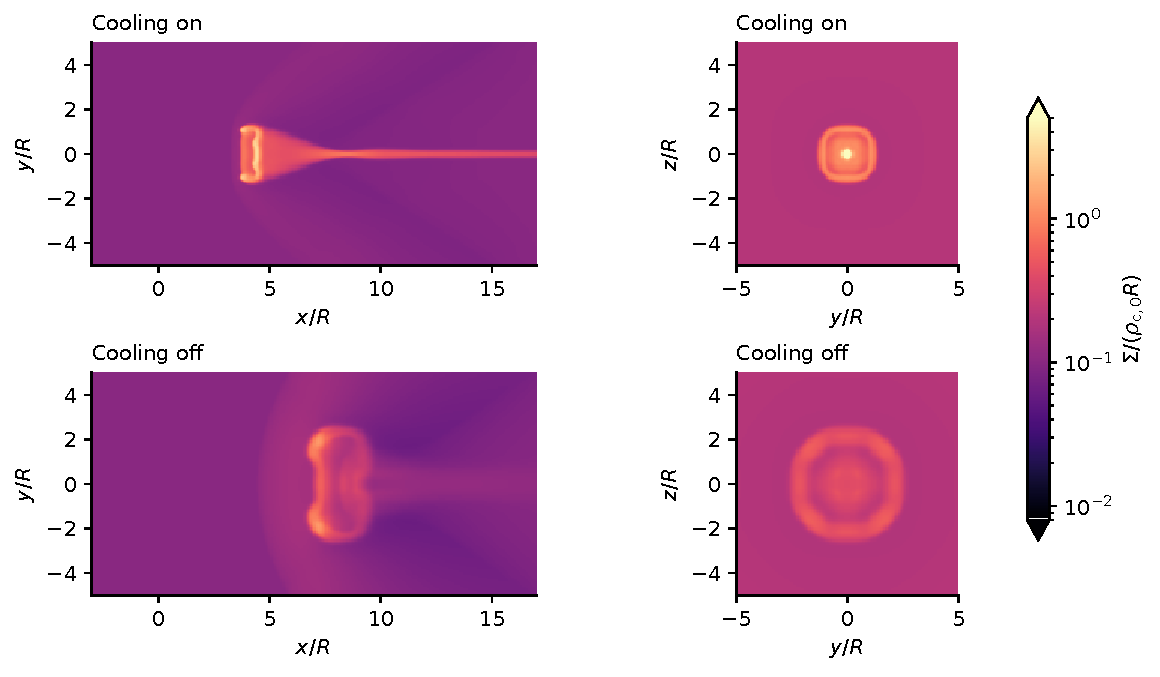
\includegraphics[width=.94\textwidth]{cooling_morphology.pdf}
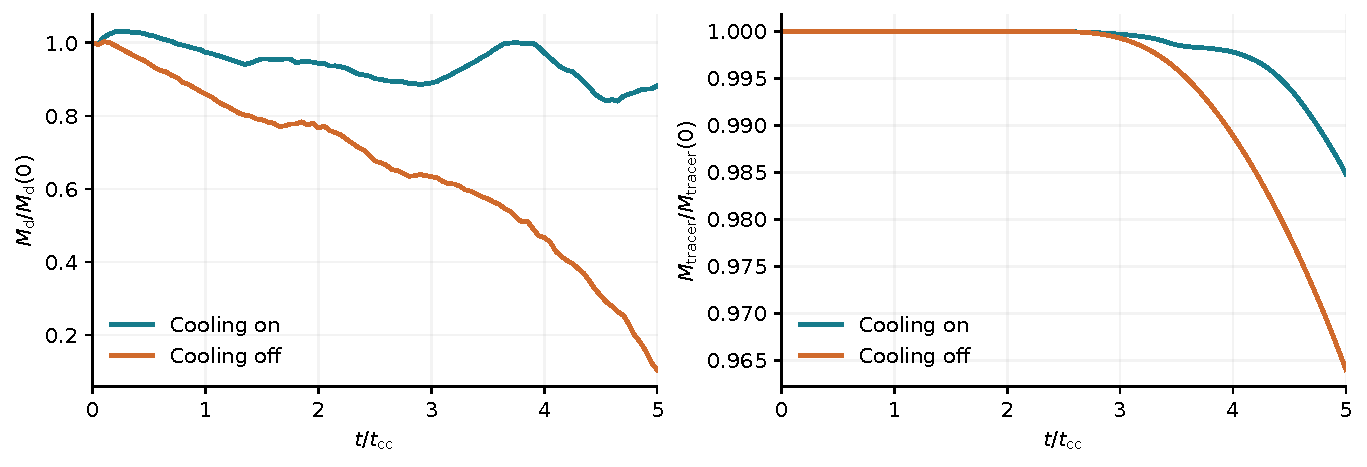
\includegraphics[width=.94\textwidth]{cooling_histories.pdf}
\caption{The supplementary AthenaPK pair at $n=128$. Upper panels show column density at $5t_{\rm cc}$ with common colour limits and viewing directions. Lower panels show dense and tagged-material masses normalized by their initial values. The initial fields and configured algorithm agree between the two runs; radiative cooling is toggled.}
\label{fig:cooling}
\end{figure*}
\begin{figure*}[tp]
\centering
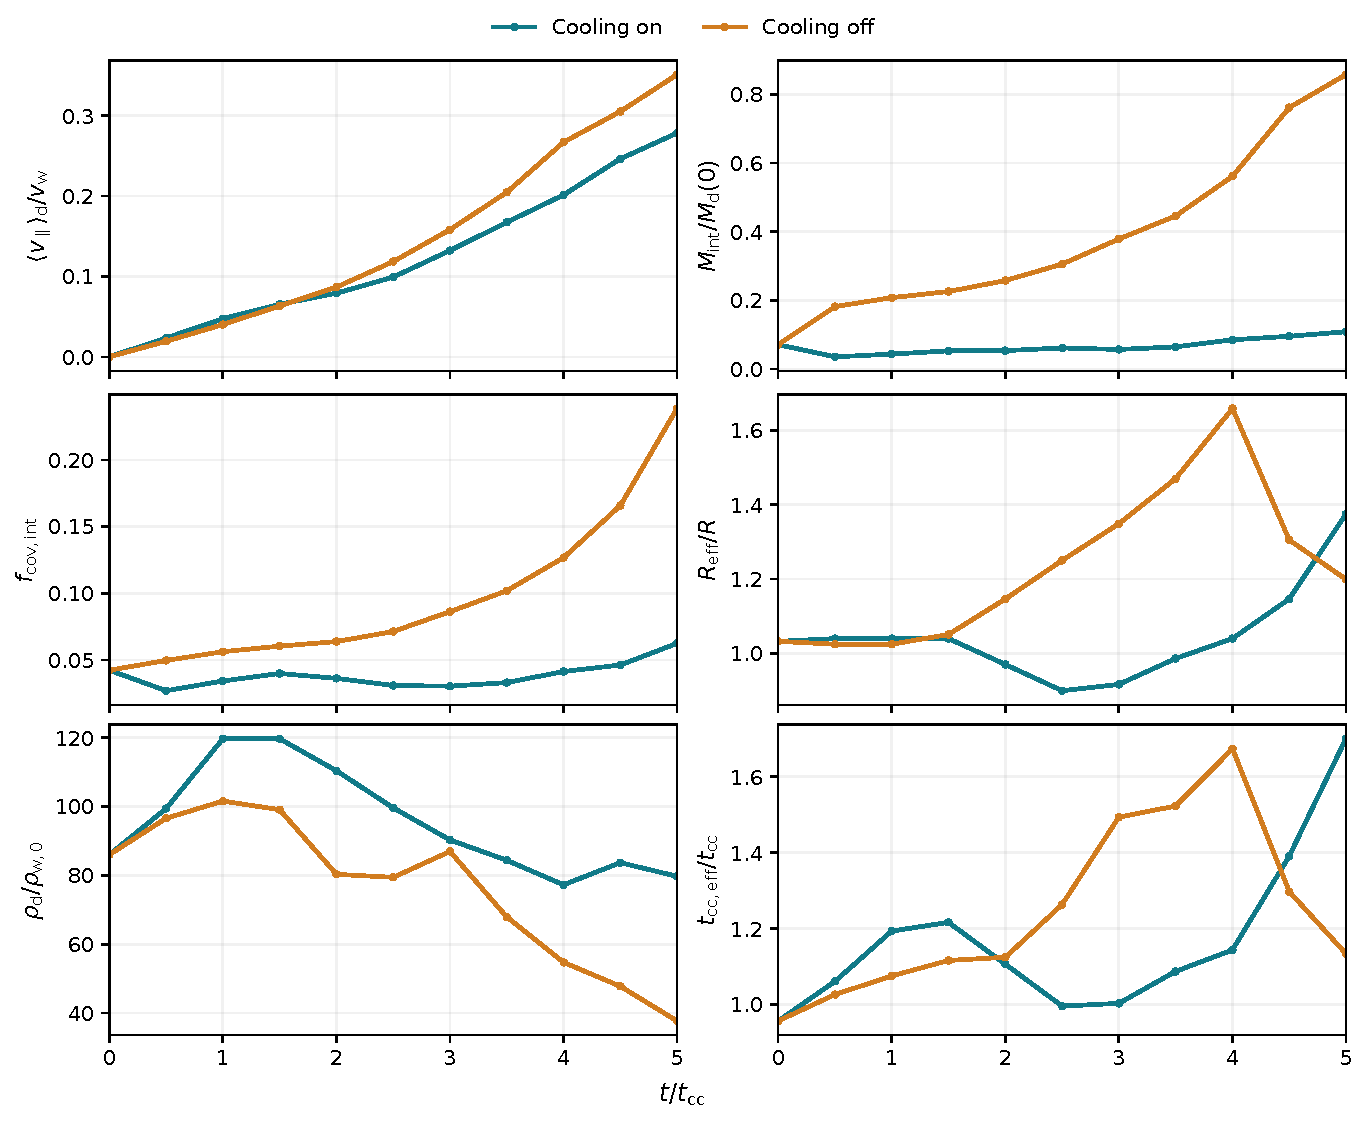
\includegraphics[width=.95\textwidth,height=.65\textheight,keepaspectratio]{cooling_diagnostics.pdf}
\caption{Additional diagnostics for the supplementary AthenaPK pair, using the same selections as Section~\ref{sec:measurements}. Their separation from the GIZMO panel preserves the distinction between the controlled cooling toggle and the non-radiative method comparison.}
\label{fig:cooldiag}
\end{figure*}

\section{Additional HLLC/PPM calculations}\label{app:hllc}
The additional AthenaPK series uses $n=128$, $\mathcal M=2$ and 101 saved states through $5t_{\rm cc}$. Table~\ref{tab:hllc} gives the accepted endpoint integrals, and Figure~\ref{fig:hllc} shows the saved dense-mass histories. Each mass is normalized by its own measured initial integral. These calculations retain the previously defined density selection and advected material tag.

\begin{table*}[tb]
\centering
\caption{Additional AthenaPK HLLC/PPM configurations at $5t_{\rm cc}$. $f_{\rm tag}$ is the tagged-material mass divided by its initial value. The final column counts global first-order fallback stages. Each row is a separately recorded source configuration.}
\label{tab:hllc}
\begin{tabular}{lrrrr}
\toprule
Configuration & $\chi$ & $f_{\rm d}$ & $f_{\rm tag}$ & Fallback stages\\
\midrule
Non-radiative & 100 & 0.1273 & 0.9816 & 17\\
Radiative & 100 & 0.9545 & 0.9878 & 282\\
Non-radiative & 10 & 0.4634 & 1.0000 & 130\\
\bottomrule
\end{tabular}
\end{table*}

The non-radiative and radiative $\chi=100$ endpoints retain 12.7 and 95.5 per cent of their initial dense masses. Both retain about 98 per cent of their original material-tag integrals. The much larger difference in dense mass therefore accompanies a change in the density distribution of retained gas. The older HLLE/PLM pilot remains a separate result, with dense fractions 0.105 and 0.882.

The new radiative calculation includes later tracer-correction source changes and a different fallback history from the non-radiative calculation. The endpoints therefore compare the recorded configurations; assigning their entire difference to cooling alone requires a pair with identical hydrodynamic source. Global first-order fallback can add diffusion, and the cooling length remains under-resolved at this sampling. The endpoint comparison establishes neither physical convergence nor a preferred hydrodynamic method.

At $\chi=10$, the HLLC/PPM dense fraction is 0.463, compared with 0.565 for the earlier HLLE/PLM configuration. The material-tag integral is retained in both. This contrast reinforces the need to distinguish a change in dense-gas membership from removal of original cloud material, and to isolate the effects of transport and correction choices in controlled comparisons.

\begin{figure*}[tp]
\centering
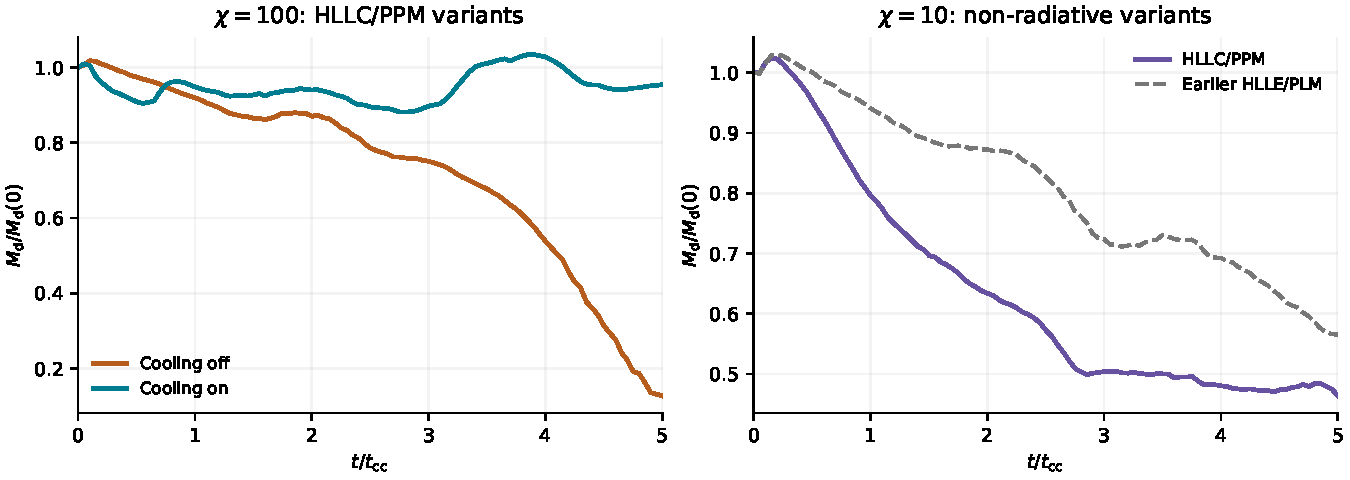
\includegraphics[width=.95\textwidth]{hllc_validated_histories_20261029.pdf}
\caption{Additional accepted scalar histories. Left: separately recorded non-radiative and radiative HLLC/PPM configurations at $\chi=100$; their correction source and fallback histories differ. Right: non-radiative $\chi=10$ numerical configurations, retaining the older HLLE/PLM curve. All calculations have $n=128$ and $\mathcal M=2$. The curves use saved numerical reductions without repeating the evolution.}
\label{fig:hllc}
\end{figure*}

\end{document}
